\documentclass[10pt]{article}

\usepackage[title]{appendix}
\usepackage{amssymb}
\usepackage{amsmath}
\usepackage[numbered,autolinebreaks]{mcode}
\usepackage{graphicx}
\usepackage{verbatim}
\usepackage[margin=1.4in]{geometry}

\newcommand*{\gam}{$\gamma \text{ }$}
\newcommand*{\gami}{$\gamma_{i} \text{ }$}
\newcommand*{\pdivq}{$\frac{p}{q} \text{ }$}

\begin{document}

\section{Introduction}

This report details the approach and implementation details relating to the first courswork project of MATH36032. Please note that all programming and testing was carried out using GNU Octave rather than MATLAB.
\section{The Euler-Mascheroni constant}

\subsection{Context}
The Euler-Mascheroni constant is a mathematical constant that first appeared in Euler's writings in 1735. It is usually denoted \gam, first appearing thus in a paper by Mascheroni in 1790 \cite{eulerconst}. Formally, it is defined as follows.

\begin{equation}
\gamma = \lim_{n \to \infty}  \left( -\ln{n} + \sum_{k=0}^{n} \frac{1}{k}  \right).
\end{equation}

Very little is known about this constant, it isn't even known whether or not it is rational. Hence it is often convenient to approximate it's value to a quotient of positive integers, which we will denote $ \frac{p}{q}$. However, if \gam is indeed irrational, for each $p$, $q$ we find, we'll be able to find another pair, who's ratio is closer to \gam. The question becomes, which integers do we choose?

Let's introduce an arbitrary integer $N$, we will aim to find a quotient of integers \pdivq such that $p + q \leq N$. Where \pdivq is the best approximation of \gam with this constraint. Furthermore, where there are multiple pairs that give the best approximation, we will take the pair with the smallest value of $p+q$.

\subsection{The brute force approach}

The approach we will to solve this problem is to first look at a brute force method. Which is to try ever possible combination of $p$ and $q$ and see which one minimises $ | \gamma - \frac{p}{q} |$. Then we will aim to optimise this approach.

  \lstinputlisting[label={bruteforce_code}, caption={A Brute force implementation to find p and q}] {../part1/AppEmBruteForce.m}

The first thing we notice about the code in Listing \ref{bruteforce_code} is it's inefficency. In Big-O notation we refer to this as being $O(N^2)$. Since an increase in $N$ results in an increase proportional to $N^2$ in the number of operations performed.

\subsection{Optimizing}
We can do better than this. The aim here, is for a given $q$, to limit the values of $p$ that we need to check. 

First lets setup some notation. Notice that in Listing \ref{bruteforce_code}, when we find a better approximation, we update the \texttt{currentBestPQ} variable. Let's denote $p_0$, $q_0$  as the first values of this variable, and $p_i$, $q_i$ to be the $i^{th}$ values of this variable. Hence the final value in this sequence is our answer. Let

\begin{equation} \label{defgammai}
  \gamma_i = \frac{p_i}{q_i}.
\end{equation}


Given a value of \gami, we know that $\gamma_{i+1}$ will be closer to the real \gam than \gami, since otherwise it wouldn't be one of the sequence. Hence

$$ |\gamma- \gamma_{i+1}| < |\gamma - \gamma_{i}| $$.

Another way of saying this is as follows. Let $\delta_{i} = | \gamma - \gamma_i  |$, then

$$ \gamma - \delta_i < \gamma_{i+1} < \gamma + \delta_i $$.

Now if we substitute equation \ref{defgammai} and multiply through by $q_{i+1}$, the result is

\begin{equation} \label{em_constraint}
q_{i+1} (\gamma - \delta_i) < p_{i+1} < q_{i+1} ( \gamma + \delta_i ).
\end{equation} 

What we have now, is for a given $q$ we have a bound on the possible values of $p$ we need to check. Furthermore, we have a way of tightening the bound every time we find a new approximation for \gam.

However, to find $\gamma_0$ currently we still have to check all possible values of $p$ when $q = 1$ since we don't yet have a current best approximation. Notice that if $N = 1,2$, though valid inputs, the results aren't useful. However, for $N \geq 3$, observe that $\gamma_0 = \frac{1}{2}$. Hence we can just hard-code this initial value. However, this does mean treating \textbf{trivial values of N} ($N = 1,2$) as a special case, but which is worth it for the saved calculations.

\emph{The reader may note at this point that it is often considered bad practice to hard-code values like this, as it sometimes effects flexiblilty. However, I argue that in this instance, we are hard-coding the value of a base case in our sequence of \gami values, and that it's performance improvement, combined with the legibility of the code makes it an acceptable approach.}

Given this justification, the code listing is as follows.

  \lstinputlisting[label={appem_code}, caption={An optimized implementation to find p and q}] {../part1/AppEm.m}

There is one further optimization in Listing \ref{appem_code} that hasn't yet been discussed. This is the constraining of $q$ as well as $p$. The reader may recall that in our brute force implementation (Listing \ref{bruteforce_code}), we allowed $q$ to run from 1 to $N$, but it's clear that $q = N$ (for non trivial values of $N$) will never contribute to the best approximation.

Let's return to equation \ref{em_constraint}. If we look at the left hand side of this constraint;

$$q_{i+1} (\gamma - \delta_i) < p_{i+1} $$,

and recall our original constraint for $p$ and $q$,
$$ p_i + q_i \leq N $$.

Combining these equation yields

$$ q_i (\gamma - \delta_i) < p_i \leq N - q_i $$ 
$$ \implies  q_i (\gamma - \delta_i) \leq N - q_i $$ 
$$ \implies q_i (\gamma - \delta_i + 1) \leq N  $$ 
$$ \implies q_i  \leq \frac{N}{(\gamma - \delta_i + 1)}  $$ 

So everytime we find a new approximation for \gam, we can also update the maximal possible value of $q$ (\texttt{qMax} in listing \ref{appem_code}). In practice this provides less of an optimization than the constraining of $p$, but for large $N$, does have a noticeable effect.

\subsection{Performance}

The performance improvement in our optimization has proven to be more than acceptable. Recall how we classified the original algorithm (Listing \ref{bruteforce_code}) to be an $O(N^2)$ algorithm. The following experiment show that the optimized version resembles an $O(N)$ time complexity. Informally, as $N$ gets larger, the time for the algorithm to terminates increases in a linear fashion.

\begin{figure}[ht]

   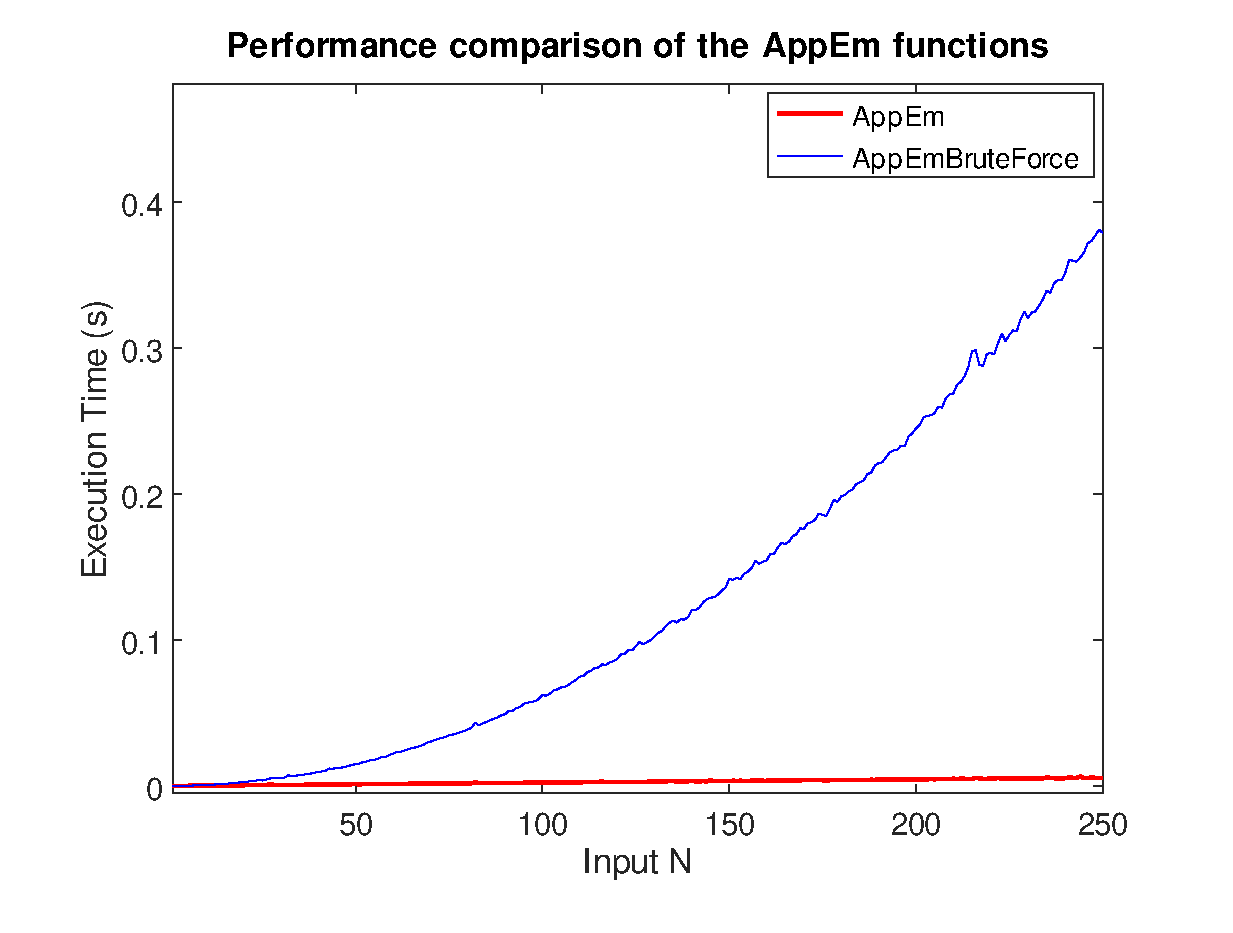
\includegraphics[scale=0.6]{bruteforce_vs_better.eps}

   \caption{A performance comparison between the brute force algorithm and the optimized version}
      \label{fig:emnaive_vs_better}
\end{figure}


Figure \ref{fig:emnaive_vs_better} shows this. It shows the time taken for both algorithms to complete for the input $N$ from 1 to 300.


\subsection{A specific example}

Let's consider the case that $N = 2019$. 

  \lstinputlisting[label={appem_test_code}, caption={A test of both implementations for N = 2019}] {../part1/part1.m}
  
Running the code in Listing \ref{appem_test_code} gives the following output

\begin{verbatim}
>> test_2019
p =  228
q =  395
Elapsed time is 0.0487769 seconds.
p =  228
q =  395
Elapsed time is 18.8509 seconds.
\end{verbatim}}

We see the output from both approaches are in agreement, and that the optimizations result in an almost 400 times speed up.

\section{Lucky numbers}

\subsection{Context}
Lucky numbers, (more commonly referred to as Carmichael numbers \cite{carmichael}) are integers $n$ that satisfy the following criterion.

\begin{enumerate}
\item The integer $n$ is not prime.
\item All the prime factors of $n$ are odd.
\item All $n$'s prime factors are distinct.
\item For each prime factor $p$ of $n$, $p - 1$ divides $n-1$ 
\end{enumerate}

Our aim is to write a function to compute the smallest lucky number which is greater than or equal to an arbitrary positive integer $N$. 

Firstly, some observations regarding the criterion.

\begin{itemize}

\item All prime factors of $n$ are odd $\iff$ $n$ is odd\\
 (since the only even prime is 2, and if $2|n$ then $n$ is even).\\
 
 Hence if $n$ is even we can immediately rule out the possibility it is lucky.
\item Given a list of the prime factors of $n$, if we find one prime factor $p$ such that $p -1 \nmid n-1$, we can rule the number isn't a lucky number, and there is no need to check the rest of the prime factors.
\end{itemize}

\subsection{The \texttt{luckynum} function}

With these observations in mind, we now aim to write a function (which we'll call \emph{luckynum}) to achieve our goal. The general approach  we will take is to check the integers greater than $N$ until we find one that's lucky. We can see at once that the first number $s$ we must check is;

$$ s = \begin{cases}
               N + 1,& \text{if N is even}\\
               N, & \text{if N is odd}
            \end{cases}
$$

Of course if this number is lucky, then we're done. But if not, what is the next number we must check? Notice that $s + 1$ must be even, since $s$ is odd by construction. We have already observed that even numbers can't be lucky. So the next number to check is $s+2$. This pattern continues as we iterate, we can increment the number being checked by 2 each time, avoiding even numbers.

The implementation of the function is as follows. 

  \lstinputlisting[label={luckynum}, caption={The luckynum function}] {../part2/luckynum.m}

What remains, is to explore how we actually check if a given number $n$ is lucky. In the \texttt{luckynum} function in Listing \ref{luckynum} we use the function \texttt{isLucky} which we will now explore.

  
\subsection{The isLucky function}

The full source is listed in Listing \ref{islucky}.
  \lstinputlisting[label={islucky}, caption={The isLucky function}] {../part2/isLucky.m}
  
The approach here is to initialise the \texttt{result} variable to true, and then as soon as one of the checks on N fails (i.e. determines N isn't lucky), result is set to false and crucially \emph{no other checks are performed}. 

First we check if $N$ is even, the reader may wonder why this is needed. Since the implementation of the \texttt{luckynum} function never calls \texttt{isLucky} with even numbers, hence this check is redundant. However we aim to produce reusable code, if we make use of the \texttt{isLucky} function in future, it may be called with an even number and so it is best practice to handle this correctly.

The order of the following checks is important, not in terms of correctness, but in terms of performance. $N$ is first factorized and the result stored. To check if the number is prime, we must only check if the number of factors is 1, which is the fastest of the operations we must perform.

Here we take advantage of \emph{lazy evaluation} to save making comparisons we don't need to. In a logical test

$$ p || q $$.

If $p$ is evaluated to be true, then Octave knows that the whole expression must be true, and doesn't evaluate $q$. So, if we have more than one prime factor, we then check if the number of prime factors is equal to the number of unique prime factors, i.e. whether there are any duplicates.

The last, and clearly slowest check is the last  of the criterion for lucky numbers. Notice that we make use of our observation that we can stop if we find any factors without the desired property in the code, in the form of a break in the loop.

The reader may notice that the most expensive operation in the implementation is the factorization of of $N$ itself and whether there are any checks we could make before this. An alternative approach is to first check if the number is prime, and only if it is not do we do the factorization. 

At first glance this seems a better solution since checking if a number is prime is faster than factorization. However, we must also consider that most numbers are not prime, so this check will fail more often than it passes, and it is in itself not a very fast operation. Hence the most common case is doing \emph{both} the factorization, and the primality check.


\begin{figure}

   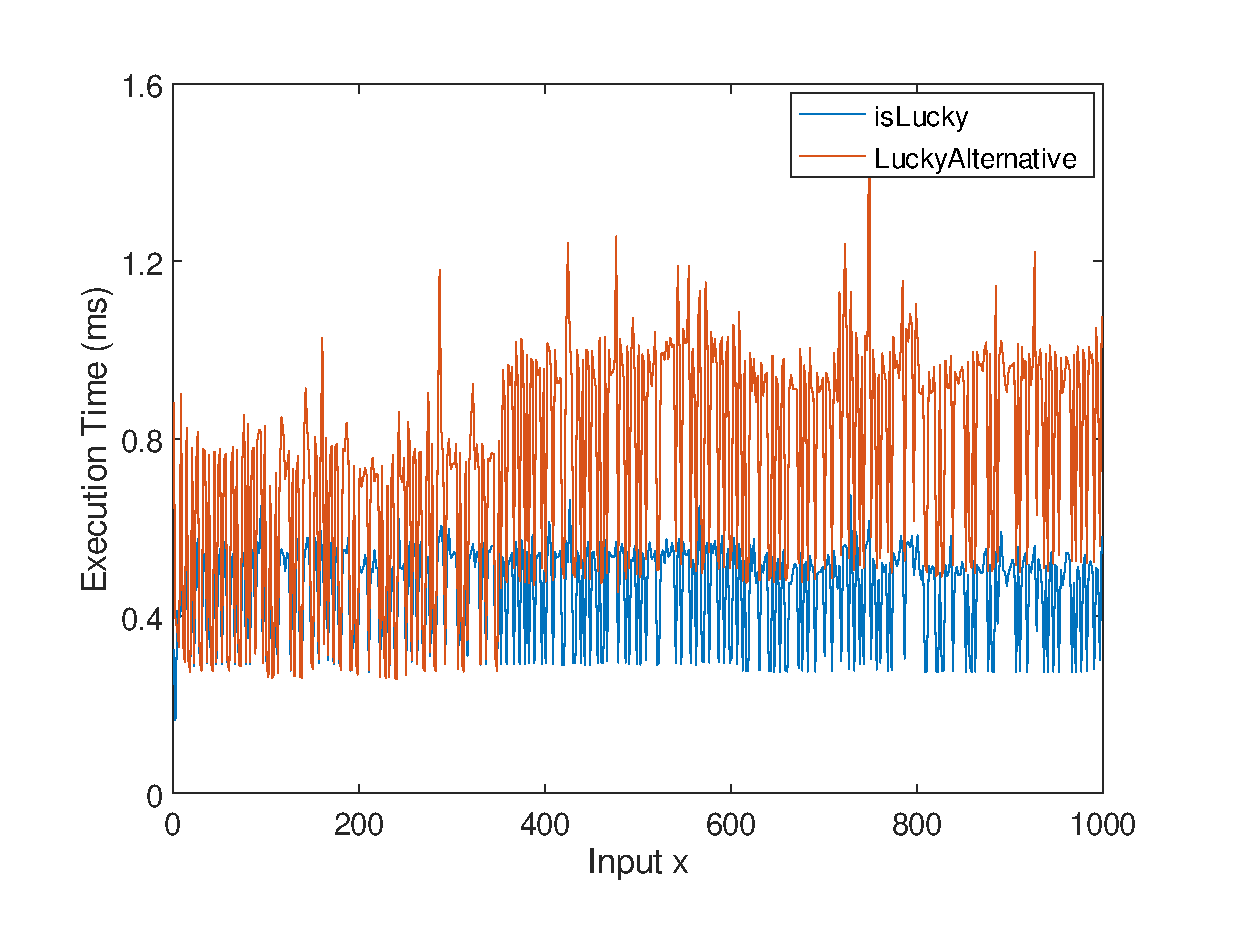
\includegraphics[scale=0.6]{islucky_test.eps}

   \caption{A performance comparison between isLucky and isLuckyAlternative. Note that the even values of x where skipped in producing the data in order to make it more legible, since both functions treat even numbers in the same way}
      \label{isluckytest}
\end{figure}


The implementation of this alternative approach is listed in Appendix \ref{islucky_appendix}, but more importantly Figure \ref{isluckytest} shows a performance comparison between the two approaches. We can see clearly that our original approach is the more efficient in the general case.

\subsection{A specific example}

The following shows the output the \emph{luckynum} function with the input of 2019.

\begin{verbatim}
>> luckynum(2019)
ans =  2465
\end{verbatim}

\section{Perfect Numbers}

\subsection{Context}
Given a positive integer $n$ we say that $n$ is \emph{perfect} if it's square consists of all the digits $1 \rightarrow 9$ exactly once. Importantly, it does \emph{not} include the digit $0$.

For example, when $ n = 24237 $

$$ n^2 = 587432169 $$

So $24237$ is said to be a perfect number.

The problem we're interested in solving is as follows, given an arbitrary integer $N$,  

\begin{equation} \label{rangeN}
10^8 < N < 10^{9}
\end{equation}


We seek the perfect number $n$ who's square is closest to $N$.

\subsection{The isPerfect function}

Firstly, we need a way of checking whether a given integer $n$ is perfect. The function is listed below (Listing \ref{isperfect}).

 \lstinputlisting[label={isperfect}, caption={The isPerfect function}] {../part3/isPerfect.m}
 
 Once again we make use of the lazy evaluation property of the language. We see that three checks are made on $n^2$
 
 \begin{itemize}
 \item Checking there are 9 digits exactly
 \item Checking that the digit $0$ doesn't appear
 \item Checking each digit appears exactly once
 \end{itemize}
 
 The checks are done in order of speed, this way, because of lazy evaluation, more expensive checks won't be carried out if cheaper checks rule out the possibility of $N$ being perfect.
 
 One thing that's been skated over so far, is the \texttt{int2Digits} function. Which returns an array of the digits of a base 10 number. (The full listing is included in Appendix \ref{int2digits}).
 
 The obvious alternative here would be to use the inbuilt \emph{num2str} function in a similar way. However, having performed some experiments comparing the two approaches, the custom approach appears to be marginally faster.
 
\subsection{The PerfNum function}

Now that we have a mechanism for determining if a given number is perfect, we can return to the original problem.

Let $n_1, n_2, ..., n_k$ be the perfect numbers in ascending order without repetitions. Our approach will be to develop an algorithm under the assumption that N lies between the squares of two perfect numbers. So suppose  for some $i \in \{ 1,..,k-1 \}$

$$ {n_i}^2 \leq N \leq {n_{i+1}}^2 $$

\emph{Then we will observe that our algorithm also returns the correct result for $N < {n_1}^2$ or $N > {n_k}^2$.} \\

Clearly, for $i<j, n_i < n_j$, so;

$$ {n_1}^2 < {n_2}^2 < ... < {n_i} ^2 \leq N \leq {n_{i+1}}^2 < ... < {n_k}^2$$

Hence by taking square roots we obtain

\begin{equation} \label{rootNbounds}
 n_1 < n_2 < ... <  n_i \leq \lfloor \sqrt{N} \rfloor \leq n_{i+1} < ... < n_k 
\end{equation}

Recall that we defined $n$ to be the perfect number who's square is closest to $N$. Clearly, by equation \ref{rootNbounds}, we know that either $n = n_i$ or $n = n_{i+1}$. 

Let $A_j =\{  \lfloor \sqrt{N} \rfloor + j,  \lfloor \sqrt{N} \rfloor  - j \} $

Now we iterate through $A_0, A_1, A_2,...$. Observe that $n \in A_j$ where $A_j$ is the first set we come across (i.e. minimal $j$) that contains a perfect number. If both elements are perfect, we take $n$ to be the one who's square is closest to $N$.

Now notice that if originally $N < {n_0}^2$, then by iterating over the sets, eventually we'll get $n_0 \in A_j$ for some j. Similarly if $N > {n_k}^2$. Hence our algorithm is guaranteed to find the correct value of $n$. \\

The code listing is below (Listing \ref{perfnum}).

 \lstinputlisting[label={perfnum}, caption={The PerfNum function}] {../part3/PerfNum.m}
 
For this function the assumption in equation \ref{rangeN} is made. Hence the worst case performance of this function is when $N$ is exactly between the squares of the two perfect numbers which have the most distance between them. We can fairly easily work out that these are $20316$ \&$22887$. 

Let's try the worst case value of $N$, which we can work out from this is $ N = 468277312 $

  \lstinputlisting[label={perfworst}] {../part3/testWorstCase.m}
  
 \begin{verbatim}
 >> testWorstCase
ans =  22887
Elapsed time is 0.959387 seconds.
\end{verbatim}

It's clear that the function in the very worst case still runs in under a second, hence for any valid input it will return in an acceptable amount of time.

\subsection{Another specific example}

The following shows the output of the \emph{PerfNum} function with the input 360322019.

\begin{verbatim}
>> PerfNum(360322019)
ans =  19023
\end{verbatim}
\begin{appendices}


\section{Alternative isLucky function}\label{islucky_appendix}

  \lstinputlisting[label={islucky_alternative}, caption={The alternative implementation of isLucky}] {../part2/isLuckyAlternative.m}
  
\section{The int2Digits function}

  \lstinputlisting[label={int2digits}, caption={The int2Digits function}] {../part3/int2Digits.m}

\end{appendices}

\begin{thebibliography}{9}
\bibitem{eulerconst}
Weisstein, Eric W. "Euler-Mascheroni Constant." From MathWorld--A Wolfram Web Resource. http://mathworld.wolfram.com/Euler-MascheroniConstant.html
Referenced: 22-02-2019

\bibitem{carmichael}
Weisstein, Eric W. "Carmichael Number." From MathWorld--A Wolfram Web Resource. http://mathworld.wolfram.com/CarmichaelNumber.html
Referenced: 23-02-2019

\end{thebibliography}

\end{document}
